%!TEX TS-program = xelatex
\documentclass[main]{subfiles}
%这是一个子文件,单独编译时会自动导入main文件的导言区
%这里可以放自定义命令,不会和别人的冲突请放心
%但是不能放newtheorem等高级命令,需要请在群里说
%下面是一些数学命令的简化,可以保留,可以删去,也可以按你的习惯修改
\def\e{\textup{e}}
\def\i{\textup{i}}
\def\T{\textup{T}}
\def\diag{\textup{diag}}
\def\id{\textup{id}}
\newcommand{\toi}[1]{{#1}\to\infty}
\newcommand{\dis}{\displaystyle}
\newcommand{\bv}{\mathrm{BV}}
\newcommand{\ac}{\mathrm{AC}}
\newcommand{\mr}{\mathbb{R}}
\newcommand{\mn}{\mathbb{N}}
\newcommand{\mq}{\mathbb{Q}}
\newcommand{\mz}{\mathbb{Z}}
\newcommand{\rel}{\text{ rel }}
\newcommand{\sgn}{\operatorname{sign}}
\newcommand{\ve}{\varepsilon}
\newcommand{\bs}{\backslash}
\renewcommand{\ll}{\lim\limits}
\renewcommand{\span}{\operatorname{span}}
\renewcommand{\ker}{\operatorname{Ker}}
\renewcommand{\hom}{\operatorname{Hom}}
\renewcommand{\leq}{\leqslant}
\renewcommand{\geq}{\geqslant}
\begin{document}
\renewcommand{\filename}{subfile11}%在这里填你的文件名,避免\label冲突
%这里开始写你的代码
%\title{No. XXX Theorem}\renewcommand\maketitlehookc{\vspace{-18ex}}\date{}
%\maketitle
\captionsetup[figure]{name={图},labelsep=period}

\section{四色定理}
\subsection{背景介绍}
每个无外飞地的地图都可以用不多于四种颜色来染色,且不会有两个邻接的区域颜色相同, 即四色定理. 这最早是Guthrie在1852年提出的猜想, 之后De Morgan致力于推动这个问题的研究工作. 1879年, Kempe发表了一个四色定理的``证明'', 当时数学界认为四色问题的猜想就此得到解决. 但在1890年, Heawood发表了一篇文章, 指出了Kempe证明中的一个错误. 虽然Heawood没能修正这个错误,但Heawood将Kempe的证明加以修改, 证明了较弱的五色定理.

证明的主要思想是,将一个含有$n$片区域的地图, 约化为不超过$n-1$片区域的地图, 从而可以证明定理成立.
之后的证明工作便成了寻找``不可避免的可约构形集'',是由Birkhoff提出的,即假设四色定理不成立, 则存在最小的不能约化的五色地图, 且最少用五种颜色染色的地图必出现某些构形, 只要再证明这些构形可以约化为区域更少的问题, 就可以推出矛盾, 最后证明四色定理. 1969年,德国数学家Heesch提出了``放电法'',
为寻找不可避免的构形提供了系统的方法. 由于人工寻找构形并验证不可约过于缓慢, Heesch试图利用计算机辅助证明. 后来, Heesch的工作被介绍到了美国. 1975年, Haken, Appel在Koch提供计算机算法的帮助下,最终得到了一个有1936个构形的不可避免构形集, 经伊利诺伊大学的主电脑``IBM 360'' 1200小时的计算, 最终证明了这些构形都是可约构形, 至此四色定理得到了成功证明. 这是首个主要借助计算机证明的定理.

\subsection{证明概述}
这里我们简述五色定理的证明, 其中的细节可参考\textbf{王敬赓《直观拓扑》}p77. Kempe证明四色定理的过程虽有误,但提供了``分构形研究''的重要思想, 这在五色定理的证明中有所体现.
\begin{lemma}
	地图染色问题中, 必存在一个区域, 与它边界相邻的区域数小于等于5.
\end{lemma}
这个引理可以利用平面图的Euler公式$V-E+F=1$证明.
\begin{theorem}[五色定理]
	每个无外飞地的地图都可以用不多于五种颜色来染色,且不会有两个邻接的区域颜色相同.
\end{theorem}
\begin{proof}
	对于一个区域数为$n$的地图,由引理, 我们只需要讨论如图1所示的四种构形. 其中a, b, c三种构形显然可以用五种颜色染色. 以c为例, 若$C_1$和$C_3$, $C_2$和$C_4$是不同的区域, 则此构形的染色问题可以约化为将$C$和$C_1$合并后的染色问题. 若$C_1$和$C_3$是同一片区域, 则可以合并$C$和$C_2$. 对于构形d, $D_1$至$D_5$中一定有两个所代表的区域是不相邻的, 不妨设为$D_1$和$D_3$, 则$D_1$和$D_3$可以染成同色, 这样构形d也可以用五种颜色染色, 此构形的染色问题可以约化为将$D$, $D_1$, $D_3$合并后的染色问题. 至此我们把原问题约化为了$n-1$或$n-2$个区域的染色问题.
	\begin{figure}[h]
		\centering
		\subfloat []
		{
			\label{fig:subfig1}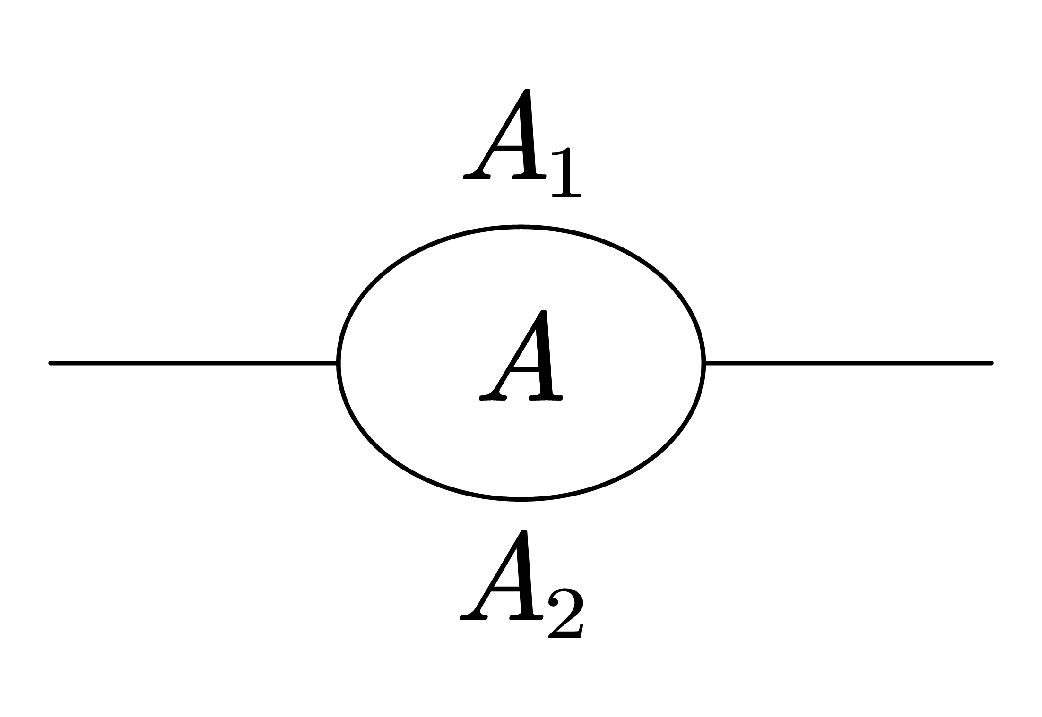
\includegraphics[width=0.2\textwidth]{Kempegraph1.pdf}
		}
		\subfloat[]
		{
			\label{fig:subfig2}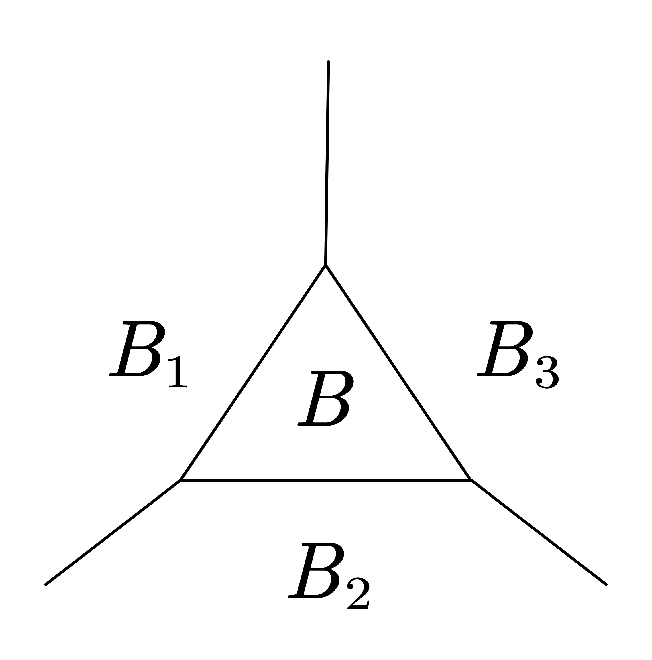
\includegraphics[width=0.2\textwidth]{Kempegraph2.pdf}
		}
		\subfloat[]
		{
			\label{fig:subfig3}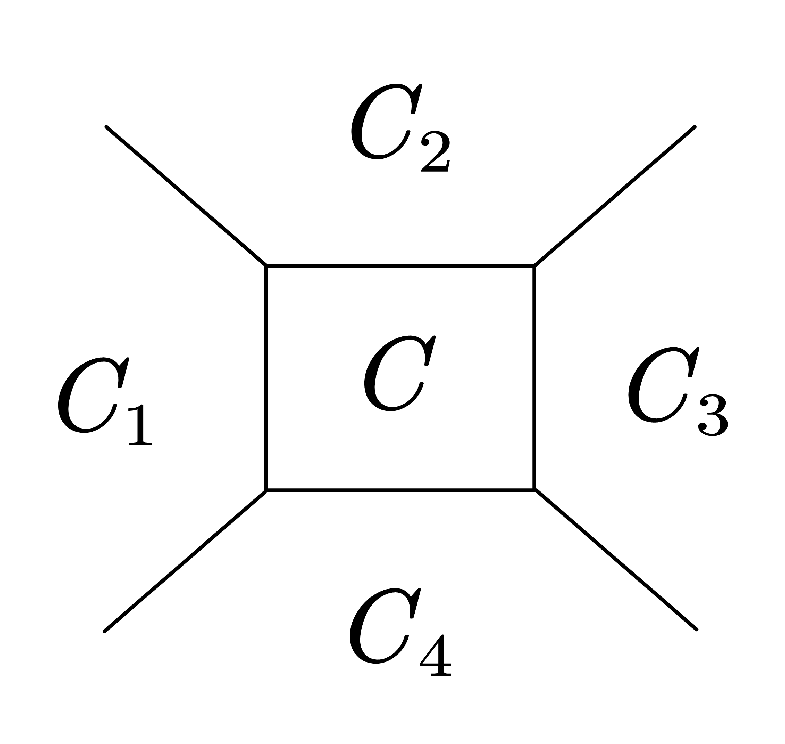
\includegraphics[width=0.2\textwidth]{Kempegraph3.pdf}
		}
		\subfloat[]
		{
			\label{fig:subfig4}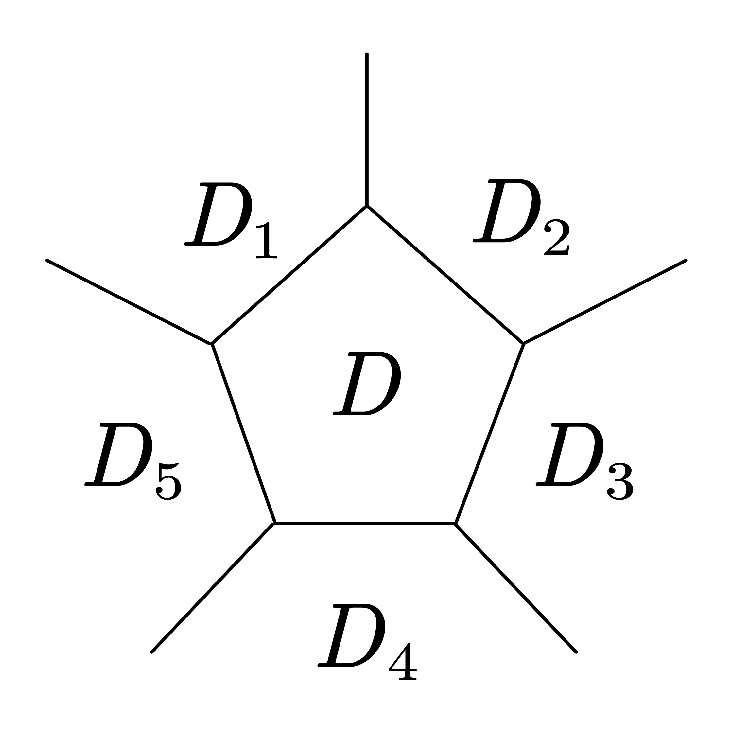
\includegraphics[width=0.2\textwidth]{Kempegraph4.pdf}
		}
		\caption{Kempe使用的不可避免构形集}
		\label{fig:subfig_1}
	\end{figure}
\end{proof}
\end{document}
